\section{Introduction}
\label{sec:introduction}

Dynamic memory management is a crucial function of programming
languages.  Correct allocation and disposal of memory regions are
fundamental for software to be reliable.

%%<<<<<<< HEAD 
%% The problem of correct dynamic memory management is challenging if a
%% programming language is equipped with manual memory management
%% primitives (e.g., \texttt{malloc} and \texttt{free} in the C
%% language.)  With such primitives, one can write a program that
%% accesses to deallocated memory regions (i.e., accesses to dangling
%% pointers) and that does not dispose memory region when it becomes
%% unnecessary (i.e., memory leak.)  In order to detect bugs related to
%% such primitives at the early stage of software development, many
%% static verification methods have been
%% proposed~\cite{DBLP:conf/aplas/SuenagaK09,DBLP:conf/pldi/HeineL03,DBLP:conf/sigsoft/XieA05,DBLP:journals/scp/SwamyHMGJ06,DBLP:conf/sas/OrlovichR06,DBLP:conf/issta/SuiYX12}.

%% This paper proposes a type-based approach to static verification of
%% memory-leak freedom that works for nonterminating programs.  Although
%% memory leaks are relatively more serious in nonterminating programs
%% (e.g., operating systems and Web servers) than terminating ones, the
%% analyses proposed so far put less emphasis to nontermination; they
%% rather verify \emph{partial} memory-leak freedom: if a program
%% terminates, then all the allocated memory cells are deallocated.  We
%% say a program is \emph{totally} memory-leak free if it does not
%% consume unbounded amount of memory during execution.
%% =======
Correct dynamic memory management is challenging if a programming
language is equipped with manual memory management primitives (e.g.,
\texttt{malloc} and \texttt{free} in the C language.)  With such
primitives, one can write a program that accesses to deallocated
memory regions (i.e., accesses to dangling pointers) and that does not
dispose memory region when it becomes unnecessary (i.e., memory leak.)
In order to detect bugs related to such primitives at the early stage
of software development, many static verification methods have been
proposed~\cite{DBLP:conf/aplas/SuenagaK09,DBLP:conf/pldi/HeineL03,DBLP:conf/sigsoft/XieA05,DBLP:journals/scp/SwamyHMGJ06,DBLP:conf/sas/OrlovichR06,DBLP:conf/issta/SuiYX12}.

This paper proposes a type-based approach to static verification of
memory-leak freedom that works for nonterminating programs.  Although
memory leaks are more serious in nonterminating programs (e.g.,
operating systems and Web servers) than terminating ones, the analyses
proposed so far put less emphasis to nontermination; they rather
verify \emph{partial} memory-leak freedom: If a program terminates,
then all the allocated memory cells are deallocated.  We say a program
is \emph{totally} memory-leak free if it does not consume unbounded
amount of memory during execution.


\begin{exmp}\label{ex:ex1}
%% Functions $h$ and $h'$ shown in Figure~\ref{ex:np} describe
%% memory-leak freedom and memory leaks in nonterminating
%% programs. Function $h$ requires two memory cells at most, whereas
%% function $h'$ requires unbounded number of memory cells to be
%% executed.
\begin{figure}[h]
1  \Rtab $h()$= \dtb \dtb\dtb\Rtab$h'()$= \\
2  \dtb $\LET \; x = \MALLOC  \; \IN$ \dtb \Rtab$\LET \; x = \MALLOC  \; \IN$\\
3  \dtb $\LET \; y = \MALLOC  \; \IN$ \dtb \Rtab$\LET \; y = \MALLOC  \; \IN$\\
4  \dtb $\Free(x)$; $\Free(y) $;\;$h()$ \dtb \Rtab$h'()$; $\Free\Cirx$; \ $\Free(y)$
\caption{Memory leaks in nonterminating programs.}
\label{ex:np}
\end{figure}
Figure~\ref{ex:np} describes partial and total memory-leak freedom.
Both \(h\) and \(h'\) are partially memory-leak free because they do
not terminate.  The function \(h\) is totally memory-leak free since
it consumes at most two cells\footnote{We assume that every memory
  cell allocated by \(\Malloc\) is fixed size.}.  However, the
function \(h'\), when it is invoked, consumes unbounded number of
memory cells; hence \(h'\) is not totally memory-leak free.
\end{exmp}

%%<<<<<<< HEAD
%% As the first step to the verification of total memory-leak freedom,
%% this paper proposes a \emph{behavioral type
%%   system}~\cite{DBLP:journals/lmcs/KobayashiSW06,DBLP:journals/tcs/IgarashiK04,DBLP:conf/esop/HondaVK98}
%% for a programming language with manual memory-management primitives.
%% Our type system captures an abstract behavior related to memory
%% allocation and deallocation as a CCS-like process.  For example, our
%% type system can assign a type \(
%% =======
As a first step to the verification of total memory-leak freedom, this
paper proposes a \emph{behavioral type
  system}~\cite{DBLP:journals/lmcs/KobayashiSW06,DBLP:journals/tcs/IgarashiK04,DBLP:conf/esop/HondaVK98}
for a programming language with manual memory-management primitives.
Our type system captures an abstract behavior related to memory
allocation and deallocation as a CCS-like process.  For example, our
type system can assign a type
\(\mu\alpha.\Malloc\TSEQ\Malloc\TSEQ\Free\TSEQ\Free\TSEQ\alpha\) to
the function \(h\) above.  This type expresses that \(h\) can allocate
a memory cell twice, deallocate a memory cell twice, and then iterate
this behavior, whereas the type assigned to \(h'\) is
\(\mu\alpha.\Malloc\TSEQ\Malloc\TSEQ\alpha\TSEQ\Free\TSEQ\Free\),
which expresses that \(h'\) can allocate a memory cell twice, call
itself recursively, and then deallocate a memory cell twice.  Hence,
by inspecting the inferred types (by using off-the-shelf model
checkers, for example), one can estimate the upper bound required to
execute \(h\) and \(h'\).

%% This way may be better than directly modelchecking the original
%% program, because we can ignore any other statements except allocation
%% and deallocation. We are now investigating some practical programs to
%% do experiments for this, and experiments are not included in our
%% paper.

One may not observe, in the example above, much difference between
applying a model checker to the original programs and to the assigned
behavioral types.  However, we expect the latter is faster than the
former in many programs because a behavioral type focuses on the
actions related to allocations and deallocations, abstracting away the
other features.  Although the current paper deals with only the
theoretical aspect, we plan to conduct experiment with actual programs
in future.

Notice that our type system alone does not prevent incorrect usage of
\(\Malloc\) and \(\Free\).  Indeed, as observed from the type assigned
to \(h\) and \(h'\) above, our types include information only about
the number and the order of allocations, deallocations, and recursive
function calls; hence, the type system does not guarantee, for
example, there is no accesses to deallocated cells.  For such
%% <<<<<<< HEAD
%% properties, we expect a program to be verified by other
%% no-illegal-access verifiers~\cite{DBLP:conf/aplas/SuenagaK09}.
%% =======
properties, we can use other no-illegal-access verifiers~\cite{DBLP:conf/aplas/SuenagaK09}.

The rest of this paper is structured as
follows. Section~\ref{sec:language} introduces a simple imperative
language and the operational semantics of the
language. Section~\ref{sec:typesystem} introduces the behavioral type
system and states the type soundness. Section~\ref{sec:reconstruction}
describes a type reconstruction procedure
Section~\ref{sec:relatedwork} discusses the related
work. Section~\ref{sec:conclusion} concludes the paper.

The proof of type soundness and the detailed definition of the type
reconstruction procedure are in the full version~\cite{fullversion}.

%% \subsection{Motivation and Problems}

%% Manual memory management primitives (e.g., \texttt{malloc} and
%% \texttt{free} in C) often cause that forgetting to deallocate memory
%% cells after use, which we call \emph{memory leaks}. It can diminish
%% the performance of the computer by reducing the amount of available
%% memory cells. Memory leaks may not be serious or even detectable by
%% normal means. Normal memory used by an application is released when
%% application terminates. This means that a memory leak in a program
%% that only runs for a short time may not be noticed and is rarely
%% serious. However, in the real-world programs, nonterminating programs
%% such as Web servers and operating systems are very important. If
%% memory leaks in such nonterminating programs, eventually, too much of
%% the available memory cells may become allocated and all or part of the
%% system stops working correctly~\cite{wiki:xxx}.

%% Most of the static analysis of memory-leak freedom proposed so
%% far~\cite{DBLP:conf/aplas/SuenagaK09,
%%   DBLP:conf/sas/OrlovichR06,DBLP:conf/pldi/HeineL03,DBLP:conf/sigsoft/XieA05,DBLP:journals/scp/SwamyHMGJ06}
%% deal with only \emph{partial memory-leak freedom}: if a program
%% terminates, allocated memory cells are all deallocated at the end. For
%% example, the type system by Suenaga and
%% Kobayashi~\cite{DBLP:conf/aplas/SuenagaK09}, which is called
%% \textbf{SK} type system in our paper, guarantees that (1) a well-typed
%% program does not conduct illegal accesses and that (2) after execution
%% of a well-typed program, all the memory cells are deallocated.

%% We tackle the problem of verifying \emph{total memory-leak freedom} in
%% this paper.\footnote{we often write memory-leak freedom for
%%   \emph{total} memory-leak freedom.} By a program being totally
%% memory-leak free, we mean that the program requires only a bounded
%% amount of memory even if it does not terminate.

%% \subsection{Approach}
%% %% <<<<<<< HEAD
%% %% =======
%% From examples in Figure~\ref{ex:np}, we notice that a simple way to guarantee memory-leak freedom for nonterminating programs is to check whether the number of allocations and deallocations is balanced before recursive call. If balanced, the program consumes bounded number of memory cells, say function $h$ allocates two memory cells and deallocates them before recursive call, it consumes two memory cells at most once; if not balanced, as function $h'$ shows, it allocates two memory cells but does not deallocate them before recursive call, which consumes unbounded number of memory cells as time goes by.
%% %% >>>>>>> 9a92815042ab957eb9b2d406af7a45d4abb729b3

%% From examples in Figure~\ref{ex:np}, we notice that a possible way to
%% guarantee memory-leak freedom for nonterminating programs is to check
%% whether the number of allocations and deallocations is balanced before
%% recursive call. If balanced, the program consumes bounded number of
%% memory cells, say function $h$ allocates two memory cells and
%% deallocates them before recursive call, it consumes two memory cells
%% at most once; if not balanced, as function $h'$ shows, it allocates
%% two memory cells but does not deallocate them before recursive call,
%% which consumes unbounded number of memory cells as time goes by.

%% To estimate the upper bound of memory consumption, we count the number
%% of allocations and deallocations by a behavioral type system. The
%% behavioral type system is mainly used to abstract the behavior of a
%% program and heavily used in the context of concurrent program
%% verification~\cite{DBLP:journals/lmcs/KobayashiSW06,DBLP:journals/tcs/IgarashiK04,DBLP:conf/esop/HondaVK98}. The
%% behavior of a program in our paper is abstracted as CCS-like
%% processes~\cite{DBLP:journals/iandc/MilnerPW92a}. For example, the
%% behavior of function $h$ is as $\mu
%% \alpha. \Malloc;\Malloc;\Free;\Free;\alpha$ which denotes it executes
%% $\Malloc$ twice, $\Free$ twice and calls itself. Similarly, the
%% behavior of $h'$ is abstracted as $\mu
%% \alpha. \Malloc;\Malloc;\alpha;\Free;\Free$.

%% One thing we should consider is like the function $f$ shown in Figure~\ref{ex:bbd}. The behavior of function $f$ is that $\Malloc$ twice, $\Free$ twice and calling itself. The abstracted behavior is $\mu \alpha. \Malloc;\Malloc;\Free;\Free;\alpha$. The number of allocation and deallocation is balanced before recursive call; the function is safe in our behavior type system, but it causes double frees: the variable $x$ is deallocated twice.
%% \begin{figure}[h]
%% 1  \Rtab\dtb\dtb $f(x)$= \\
%% 2  \dtb \dtb\dtb$\LET \; x = \MALLOC  \; \IN$ \\
%% 3  \dtb \dtb\dtb$\LET \; y = \MALLOC  \; \IN$ \\
%% 4  \dtb \dtb\dtb$\Free(y)$; $\Free(y) $;\;$f(x)$
%% \caption{balanced but double free}
%% \label{ex:bbd}
%% \end{figure}

%% Thanks to the \textbf{SK} type system, proposed by Suenaga and Kobayashi, it guarantees no double frees or illegal access to a deallocated memory cell. By combining the \textbf{SK} type system, our behavior type system can ignore the relationship between variables and pointers, so to estimate the upper bound of consumption memory cells according to the abstraction of the behavior of programs is sound.

%% \subsection{Overview of the algorithm}

%% \begin{figure}
%%  \centering
%% 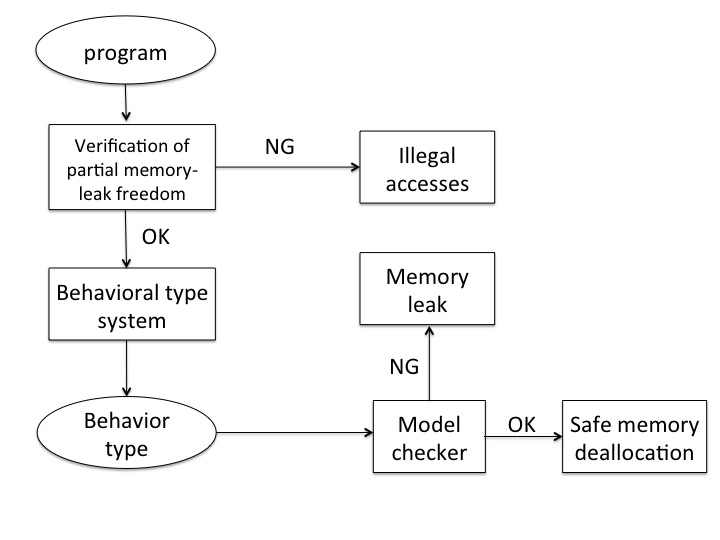
\includegraphics[width=10cm]{overview.jpg}
%% \caption{Overview of the algorithm}
%% \label{fig:ov}
%% \end{figure}

%% %% <<<<<<< HEAD
%% %% A program is first checked by $\mathbf{SK}$ type system; it is passed
%% %% to the behavioral type system proposed in our paper if its partial
%% %% correctness is guaranteed, otherwise returns ``it is not safe''; the
%% %% behavioral type system will check it and produce a behavioral type $P$
%% %% which abstracts the behavior of the program; and then by modeling the
%% %% behavioral type $P$ using model checkers like \texttt{SPIN} or
%% %% \texttt{CPAChecker} to verify whether the behavioral correctness of
%% %% the program is guaranteed. If its behavioral correctness is verified
%% %% by model checker, the safe memory deallocation for this program is
%% %% ensured, otherwise return ``it is not safe''.
%% %% =======
%% As represented in Figure~\ref{fig:ov}, a program is first checked by \textbf{SK} type system; if the properties about no double frees or illegal read/write operations to a deallocated memory cell is guaranteed, then it returns ``OK'' and the program is passed to our behavior type system, and it returns ``NG'' otherwise; our behavior type system will produce a behavioral type, and this behavioral type is passed to a model checker like \texttt{SPIN} or \texttt{CPAChecker} to verify whether it is consumed upper bound of memory cells.

%% Hence, by using our type system with \textbf{SK} type system, we can verify memory-leak freedom even for nonterminating programs.
%% %% >>>>>>> 9a92815042ab957eb9b2d406af7a45d4abb729b3

\paragraph{Notation} We write \(\vec{X}\) for a finite sequence of
\(X\).  We write \([\vec{x'}/\vec{x}]s\) for the term obtained by
replacing every free occurrences of \(\vec{x}\) in \(s\) with
\(\vec{x'}\).  We write \(\DOM(f)\) for the domain of the map \(f\).  For a
map \(f\), we write \(f \set{x \mapsto v}\) and \(f \bs x\) for the
maps defined as follows:
\[
\begin{array}{rcl}
f \set{x \mapsto v} (w) &=&
\left\{
\begin{array}{ll}
v & \mbox{if \(x = w\)}\\
f(w) & \mbox{otherwise.}
\end{array}
\right.\\
(f \bs x)(w) &=&
\left\{
\begin{array}{ll}
\mbox{undefined} & \mbox{if \(w \in \DOM(f)\)}\\
f(w) & \mbox{otherwise.}
\end{array}
\right.
\end{array}
\]
